\documentclass[cjk,dvipdfmx,12pt,%
hyperref={bookmarks=true,bookmarksnumbered=true,bookmarksopen=false,%
colorlinks=false,%
pdftitle={Debian GNU/kFreeBSDで暮らせる環境を構築してみる},%
pdfauthor={杉本典充},%
%pdfinstitute={dictoss@live.jp},%
pdfsubject={第38回関西Debian勉強会},%
}]{beamer}

\title{Debian GNU/kFreeBSDで暮らせる環境を構築してみる}
\subtitle{{\scriptsize{$\sim$第38回関西Debian勉強会$\sim$}}}
\author[杉本 典充]{{\large\bf 杉本典充}}
\institute[]{{\normalsize\tt dictoss@live.jp}}
\date{{\small 2010 年 8 月 22 日}}

%\usepackage{amsmath}
%\usepackage{amssymb}
\usepackage{graphicx}
\usepackage[varg]{txfonts}
%\usepackage{D6math}
\AtBeginDvi{\special{pdf:tounicode EUC-UCS2}}
\usetheme{Kyoto}
\def\museincludegraphics{%
  \begingroup
  \catcode`\|=0
  \catcode`\\=12
  \catcode`\#=12
  \includegraphics[width=0.9\textwidth]}
%\renewcommand{\familydefault}{\sfdefault}
%\renewcommand{\kanjifamilydefault}{\sfdefault}
\begin{document}
\settitleslide
\begin{frame}
\titlepage
\end{frame}
\setdefaultslide


\begin{frame}[fragile]
\frametitle{発表において}
\begin{itemize}
  \item 何か質問、疑問があれば随時質問をどうぞ。
  \item ツッコミ、大歓迎。間違いを指摘していただくとこの場の皆さんが
幸せになれます。
\end{itemize}
\end{frame}


\begin{frame}[fragile]
\frametitle{アジェンダ}
\begin{itemize}
  \item 自己紹介
  \item Debian GNU/kFreeBSDとは
  \item Debian GNU/kFreeBSDの環境構築
  \begin{itemize}
    \item インストール
    \item カーネルの更新
    \item xorg、デスクトップ環境
    \item 日本語環境
    \item 開発環境
    \item デバイスドライバの導入
  \end{itemize}
  \item 終わりに
  \item 質問コーナー
\end{itemize}
\end{frame}


\begin{frame}[fragile]
\frametitle{発表者について}
\begin{itemize}
  \item 名前:杉本 典充 (dictoss@live.jp)
  \item Twitter : dictoss
  \item Debian GNU/Linuxは大学2年の頃から使っている。
(当時はtestingのsarge)
  \item ここ数年Debian GNU/LinuxとFreeBSDを集中して使っている。
  \item Debian GNU/kFreeBSDという神OSが降臨してきたことを知り、
使い始めたのが昨年。
\end{itemize}
\end{frame}


\begin{frame}[fragile]
\frametitle{Debian GNU/kFreeBSDとは}
\begin{itemize}
  \item Debian Projectで開発が進んでいる新しいOS。
  \item カーネルはFreeBSDカーネルを使用。
  \item パッケージシステムはdpkg/apt。
  \item 採用ソフトウェアはDFSGに従って決定する。
  \item 現段階ではi386版とamd64版の2つのアーキテクチャをサポート。
  \item 主な情報はDebian Wikiにある。(英語なのでかんばって読みましょう。)
\end{itemize}
\end{frame}


\begin{frame}[fragile]
\frametitle{Debian GNU/kFreeBSDとDebian GNU/Linuxの違い(1)}
\begin{itemize}
\item デバイスドライバ系
  \begin{itemize}
  \item サウンドデバイスはOSS。
  \item eth0は存在しません。(このマシンはem0で認識しています)
  \item ディスクデバイス名は「/dev/ad4s1」(内蔵HDD)や
「/dev/da0s1」(USBメモリ)として認識する。
  \item mount系コマンドが/sbinの下にたくさんあったり、
オプションが若干異なります。
  \end{itemize}
\end{itemize}
\end{frame}


\begin{frame}[fragile]
\frametitle{Debian GNU/kFreeBSDとDebian GNU/Linuxの違い(2)}
\begin{itemize}
\item ファイルシステム系
  \begin{itemize}
  \item 現時点ではUFS、ext2が使用可能。
  \item ext3は読み込みのみ可能。
  \item 昨日Debian Wikiを確認したら、zfsutilsというパッケージが追加されて、ZFSが使えるようになった模様。(/パーティションをZFSにできるかは不明。)
  \end{itemize}
\end{itemize}
\end{frame}


\begin{frame}[fragile]
\frametitle{Debian GNU/kFreeBSDとDebian GNU/Linuxの違い(3)}
\begin{itemize}
\item 仮想化
  \begin{itemize}
  \item FreeBSDといえばJail。(chrootの拡張です。)
  \item VirtualBox (Debianパッケージとしてあるが・・・。)
  \item QEMU
  \end{itemize}
\end{itemize}
\end{frame}


\begin{frame}[fragile]
\frametitle{インストール}
\begin{itemize}
  \item インストーラはdailyビルドがあるのでダウンロードする。
  \item 今回はi386版をインストールしました。
\end{itemize}
\begin{center}
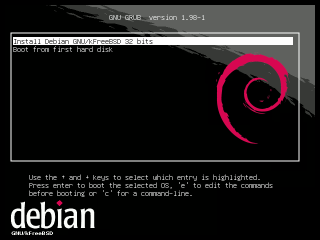
\includegraphics[scale=0.5]{image201008/kfreebsd-installer.png}
\end{center}
\end{frame}


\begin{frame}[fragile]
\frametitle{カーネルの更新(1)}
\begin{commandline}
$ uname -a
GNU/kFreeBSD deb-NorTP60 7.3-1-686 #0
Tue Jul 20 02:12:21 CEST 2010 i686 i386
Genuine Intel(R) CPU           T2400  @ 1.83GHz GNU/kFreeBSD
\end{commandline}
\begin{commandline}
$ cat /proc/cpuinfo
processor   : 0
vendor_id   : GenuineIntel
cpu family  : 6
model       : 7
model name  : Genuine Intel(R) CPU           T2400  @ 1.83GHz
stepping    : 8
flags       : fpu vme de pse tsc msr pae mce cx8 apic sep mtrr pge mca
              cmov pat b19 b21 mmxext mmx fxsr xmm b26 b27 b28 b29 3dnow
cpu MHz     : 1828.76
bogomips    : 1828.76
\end{commandline}
インストール直後はCPUが1個しか認識していない。
\end{frame}


\begin{frame}[fragile]
\frametitle{カーネルの更新(2)}
\begin{commandline}
$ apt-cache search kfreebsd-image-*
kfreebsd-image-7-486 - kernel of FreeBSD 7 image
kfreebsd-image-7-686-smp - kernel of FreeBSD 7 image
kfreebsd-image-7-686 - kernel of FreeBSD 7 image
kfreebsd-image-7.3-1-486 - kernel of FreeBSD 7.3 image
kfreebsd-image-7.3-1-686-smp - kernel of FreeBSD 7.3 image
kfreebsd-image-7.3-1-686 - kernel of FreeBSD 7.3 image
kfreebsd-image-8-486 - kernel of FreeBSD 8 image
kfreebsd-image-8-686-smp - kernel of FreeBSD 8 image
kfreebsd-image-8-686 - kernel of FreeBSD 8 image
kfreebsd-image-8.0-1-486 - kernel of FreeBSD 8.0 image
kfreebsd-image-8.0-1-686-smp - kernel of FreeBSD 8.0 image
kfreebsd-image-8.0-1-686 - kernel of FreeBSD 8.0
\end{commandline}
\begin{commandline}
$ sudo apt-get install kfreebsd-image-7.3-1.686-smp
$ sudo reboot
\end{commandline}
\end{frame}


\begin{frame}[fragile]
\frametitle{カーネルの更新(3)}
\begin{commandline}
$ uname -a
GNU/kFreeBSD deb-NorTP60 7.3-1-686-smp #0
Tue Jul 20 02:43:20 CEST 2010 i686 i386
Genuine Intel(R) CPU           T2400  @ 1.83GHz GNU/kFreeBSD
\end{commandline}
\begin{commandline}
$ cat /proc/cpuinfo
processor   : 0
vendor_id   : GenuineIntel
model name  : Genuine Intel(R) CPU           T2400  @ 1.83GHz
processor   : 1
vendor_id   : GenuineIntel
model name  : Genuine Intel(R) CPU           T2400  @ 1.83GHz
stepping    : 8
flags       : fpu vme de pse tsc msr pae mce cx8 apic sep mtrr pge mca
              cmov pat b19 b21 mmxext mmx fxsr xmm b26 b27 b28 b29 3dnow
\end{commandline}
CPUが2個使えるようになりました。
\end{frame}


\begin{frame}[fragile]
\frametitle{Xorg}
\begin{commandline}
$ sudo apt-get install xorg
Setting up hal (0.5.14-3) ...
Reloading system message bus config...
Failed to open connection to ``system'' message bus:
Failed to connect to socket /var/run/dbus/system_bus_socket: Connection refused
invoke-rc.d: initscript dbus, action ``force-reload'' failed.
Starting Hardware abstraction layer: haldinvoke-rc.d: initscript hal,
action ``start'' failed.
dpkg: error processing hal (--configure):
 subprocess installed post-installation script returned error exit status 1
\end{commandline}

どうやら既知バグの模様で未解決状態。

http://bugs.debian.org/cgi-bin/bugreport.cgi?bug=469528
\end{frame}


\begin{frame}[fragile]
\frametitle{Xorg}
\begin{itemize}
  \item 原因はhalの後処理で実行する「/etc/init.d/dbus reload」でエラーが
発生した模様。
  \item dbusが停止しているので「/etc/init.d/dbus start」で起動した。
  \item 再度「apt-get install xorg」。
  \item また失敗したが少し進んだので、再度「/etc/init.d/dbus start」。
  \item とりあえずxorgをインストールできた。
  \item xorg.confがないので新規に生成して、/etc/X11/xorg.confに配置。
  \item startxも成功したのでとりあえずOKとする。
\end{itemize}
\end{frame}

\begin{frame}[fragile]
\frametitle{gdm}
\begin{itemize}
  \item インストール自体は成功。
  \item 再起動するとキーボード入力ができない!!
  \item 仕方がないのでgdmでのログインは諦める。
  \item gdmのpurgeに一苦労。
\end{itemize}
\end{frame}

\begin{frame}[fragile]
\frametitle{デスクトップ環境}
\begin{commandline}
$ sudo apt-get install xfce4 xfce4-goodies
\end{commandline}

\begin{commandline}
$ vim ~/.xinitrc
exec xfce4-session

$ chmod 744 ~/.xinitrc
$ startx
\end{commandline}

無事にXfce4が起動できた。
\end{frame}

\begin{frame}[fragile]
\frametitle{日本語環境}
\begin{commandline}
$ sudo apt-get install otf-ipafont otf-ipaexfnt
$ sudo apt-get install locales-all
$ sudo apt-get install uim uim-anthy
\end{commandline}

\begin{commandline}
$ vim ~/.xinitrc
export LANGUAGE='ja_JP.UTF-8'
export LC_ALL='ja_JP.UTF-8'
export LANG='ja_JP.UTF-8'

export XMODIFIRES='@im=uim'
export GTK_IM_MODULE='uim'
export QT_IM_MODULE='uim'

exec xfce4-session

$ startx
\end{commandline}

日本語の表示、入力は問題なく可能です。
\end{frame}

\begin{frame}[fragile]
\frametitle{開発環境}
\begin{commandline}
$ sudo apt-get install gcc  g++ gdb make
$ sudo apt-get install build-essential pbuilder debian-keyring
\end{commandline}

試しにtcshをビルドしてみる。
\begin{commandline}
$ apt-get source tcsh
$ sudo apt-get build-dep tcsh
$ cd tcsh-6.17.00
$ dch
$ debuild -i -us -uc -b
$ sudo dpkg -i tcsh_6.17.00-3.1_kfreebsd-i386.deb
\end{commandline}

debパッケージのビルド、インストールができました。
\end{frame}

\begin{frame}[fragile]
\frametitle{Debian勉強会資料のビルド環境(1)}
\begin{itemize}
  \item contrib, non-freeのパッケージが必要なため、apt-lineを修正。
\end{itemize}
\begin{commandline}
$ sudo vim /etc/apt/sources.list
deb http://ftp.jp.debian.org/debian/ squeeze main contrib non-free
deb-src http://ftp.jp.debian.org/debian/ squeeze main contrib non-free

deb http://security.debian.org/ squeeze/updates main
deb-src http://security.debian.org/ squeeze/updates main
\end{commandline}
\begin{commandline}
$ sudo apt-get install git-core
$ sudo apt-get install gs gs-esp gs-cjk-resource
$ sudo apt-get install ptex-bin xdvik-ja dvipsk-ja
$ sudo apt-get install okumura-clsfiles vfdata-morisawa5
$ sudo apt-get install texlive-latex-extra
$ sudo apt-get install poppler-data
$ sudo apt-get install evince
\end{commandline}
\end{frame}


\begin{frame}[fragile]
\frametitle{Debian勉強会資料のビルド環境(2)}
\begin{commandline}
$ cd
$ git clone git://git.debian.org/git/tokyodebian/monthly-report.git/
$ cd monthly-report
$ make
\end{commandline}
\end{frame}


\begin{frame}[fragile]
\frametitle{日常生活に必要なソフトウェアのインストール}
\begin{commandline}
$ sudo apt-get install emacs emacs23-el
$ sudo apt-get install sylpheed sylpheed-i18n
$ sudo apt-get install iceweasel iceweasel-l10n-ja
$ sudo apt-get install audacious audacity
$ sudo apt-get install gxine
$ sudo apt-get install jd
$ sudo apt-get install gftp
\end{commandline}
\end{frame}

\begin{frame}[fragile]
\frametitle{サウンドドライバのロード(1)}
mp3のサウンドファイルを再生するが音が鳴らない・・・。

サウンドドライバを確認し、ロードします。
\begin{commandline}
$ kldstat
 1   10 0xc0400000 890000   kfreebsd-7.3-1-686-smp.gz
 2    1 0xc0d9c000 57fdc    acpi.ko
 3    1 0xc5c7a000 67000    radeon.ko
 4    1 0xc5ce1000 14000    drm.ko
\end{commandline}
\begin{commandline}
$ sudo kldload snd_hda
$ kldstat
 1   10 0xc0400000 890000   kfreebsd-7.3-1-686-smp.gz
 2    1 0xc0d9c000 57fdc    acpi.ko
 3    1 0xc5c7a000 67000    radeon.ko
 4    1 0xc5ce1000 14000    drm.ko
 5    1 0xc611f000 1a000    snd_hda.ko
 6    1 0xc6139000 40000    sound.ko
\end{commandline}
\end{frame}

\begin{frame}[fragile]
\frametitle{サウンドドライバのロード(2)}
再起動すると、サウンドドライバが自動ロードされないので設定します。

\begin{commandline}
$ sudo vim /etc/modules
# /etc/modules: kernel modules to load at boot time.
#
# This file should contain the names of kernel modules that are
# to be loaded at boot time, one per line.  Comments begin with
# a ``#'', and everything on the line after them is ignored.
snd_hda.ko
\end{commandline}

各種カーネルモジュール(*.ko)は、

/lib/modules/7.3-1-smp ディレクトリの下にあります。

(kfreebsd-image-7.3-1-smpのカーネルの場合)
\end{frame}

\begin{frame}[fragile]
\frametitle{今後の課題}
\begin{itemize}
  \item Flashの再生環境
  \begin{itemize}
    \item Abobe公式のFreeBSD版バイナリはない。
    \item 昨日時点でgnashのパッケージが追加されていた。
入れたけど動かなかったので動かす方法を探してみます。
  \end{itemize}
  \item ビデオ再生の品質が悪い。(codecか?)
  \item Linuxバイナリ互換機能
  \item 仮想化機能
  \item ZFS
\end{itemize}
\end{frame}

\begin{frame}[fragile]
\frametitle{環境構築を終えて}
\begin{itemize}
  \item Debianインストーラも整備されインストールしやすい。
  \item Debian GNU/kFreeBSDもDebian GNU/Linuxも同じDebianなので少し慣れればOK。
  \item ただ、日が浅いOSなのでトラブルが起こるとFreeBSDカーネルの問題なのか、
Debianシステムの問題なのか、切り分けに時間がかかる。
  \item BTSは貴重な情報源。
  \item Debian GNU/kFreeBSDはSqueezeで技術プレビューとして公開予定。
\end{itemize}
\end{frame}


\begin{frame}[fragile]
\frametitle{参考文献}
\begin{itemize}
\item \url{http://tokyodebian.alioth.debian.org/pdf/debianmeetingresume201006-iwamatsu-presentation.pdf}
\item \url{http://wiki.debian.org/Debian_GNU/kFreeBSD_FAQ}
\end{itemize}
\end{frame}


\end{document}
%%% Local Variables: 
%%% mode: japanese-latex
%%% TeX-master: t
%%% End: 
